\documentclass[mingoth,11pt,a4j,uplatex,dvipdfmx]{jsarticle}
\usepackage[top=20truemm,bottom=20truemm,left=20truemm,right=20truemm]{geometry}
\usepackage{moreverb}
\usepackage{listings,jlisting} %日本語のコメントアウトをする場合jlistingが必要
								% https://qiita.com/N_Matsukiyo/items/1199f07a0e1bf4fce29c
\usepackage[dvips]{graphicx,color}

% https://qiita.com/ta_b0_/items/2619d5927492edbb5b03
\lstset{
  basicstyle={\ttfamily},
  identifierstyle={\small},
  commentstyle={\smallitshape},
  keywordstyle={\small\bfseries},
  ndkeywordstyle={\small},
  stringstyle={\small\ttfamily},
  frame={tb},
  breaklines=true,
  columns=[l]{fullflexible},
  numbers=left,
  xrightmargin=0zw,
  xleftmargin=3zw,
  numberstyle={\scriptsize},
  stepnumber=1,
  numbersep=1zw,
  lineskip=-0.5ex
}


\renewenvironment{description}%  descriptionをインデント
{%
   \begin{list}{\parbox{1zw}{$\bullet$}}% 見出し記号/直後の空白を調節
   {%
      \setlength{\topsep}{1zh}
      \setlength{\itemindent}{3zw}
      \setlength{\leftmargin}{5zw}%  左のインデント
      \setlength{\rightmargin}{0zw}% 右のインデント
      \setlength{\labelsep}{1zw}%    黒丸と説明文の間
      \setlength{\labelwidth}{3zw}%  ラベルの幅
      \setlength{\itemsep}{0em}%     項目ごとの改行幅
      \setlength{\parsep}{0em}%      段落での改行幅
      \setlength{\listparindent}{0zw}% 段落での一字下り
   }
}{%
   \end{list}%
}

\title{float / flexbox / css grid}
\date{\today}

\setcounter{secnumdepth}{3}
\setcounter{tocdepth}{3}

\begin{document}
%\gtfamily	%全てゴシックに

\maketitle

\begin{abstract}
float / flexbox / css gridの違いについて学び、今時のレイアウト方法を学ぼう
\end{abstract}

\tableofcontents
\newpage

\section{はじめに}
\subsection{読み間違えないでね}

\begin{lstlisting}[caption=読み間違えないでね]
数字:0123456789
小文字:abcdefghijklmnopqrstuvwxyz
大文字:ABCDEFGHIJKLMNOPQRSTUVWXYZ

1:イチ
l:小文字のエル
i:小文字のアイ
!:ビックリマーク
|:バーティカルバー。Shiftと¥を押したもの。

0:ゼロ
o:小文字のオー
O:大文字のオー

.:ピリオド
,:コンマ
\end{lstlisting}

\subsection{注意}
\begin{itemize}
\item これから出てくるソースコードには、左に「行番号」と呼ばれる番号が出てくるけど、入力する必要ないからね。
\end{itemize}

\section{floatはレイアウトを組むのには厄介!}
\subsection{VSCodeのちょっとした機能 lorem ipsum}
floatに入る前にlorem ipsumについて説明します。

出版、ウェブデザイン、グラフィックデザインなどの諸分野において使用されている典型的なダミーテキストのことをlorem ipsum(ローレムイプサム)と言います。ダミーテキストのため、意味は全くありません。(一応、もとは古代ローマの政治家・哲学者キケロの『De finibus bonorum et malorum』(善と悪の究極について)という著作から取られている。)

vscodeでは、lorem10, lorem20, lorem30等と入力してリターンを押すことによって、その単語数分の文字を自動で入力してくれます。

以下の例では、lorem10, lorem20, lorem30, lorem50を利用しています。



\subsection{id08-float.html}
どうなるか想像しながら入力してみよう。
\begin{lstlisting}[caption=HTML部分]
<!DOCTYPE html>
<html>
	<head>
		<meta charset="UTF-8">
		<title>float</title>
	</head>
	<body>
    		<div class="columns">
		        <div class="child">
		            Lorem ipsum dolor sit amet consectetur adipisicing elit. Asperiores, eum?
		        </div>
		        <div class="child">
		            Lorem ipsum dolor sit amet consectetur, adipisicing elit. Dolores facere numquam assumenda delectus totam nam nisi accusamus est illum expedita!
		        </div>
		        <div class="child">
		            Lorem ipsum dolor sit amet consectetur adipisicing elit. Debitis vel ducimus impedit omnis esse velit est, quo at modi maxime tempore dicta labore beatae ipsa minima maiores aut quisquam animi!
		        </div>
		 </div>
		 <div>
			<p>
				Lorem ipsum dolor sit amet consectetur adipisicing elit. Dolor natus reprehenderit voluptate ab non molestias incidunt corrupti, distinctio, nobis quidem tempore rerum facere perferendis atque harum quisquam magni facilis fugit veniam possimus perspiciatis ea accusantium odit quia. Nam aliquid ea quod dolorem impedit asperiores! Amet quam sequi optio vitae consectetur!
			</p>
		</div>
	</body>
</html>
\end{lstlisting}


\subsection{childクラスにスタイルを当ててみよう}
headタグの中に次のCSSを入れて見てみよう。入力する前にどんな感じになるか考えてみよう。
\begin{lstlisting}[caption=CSS部分1]
    <style>
        .child {
            border: 1px solid black;
            float: left;
            width: 25%;
            padding: 10px;
            margin-right: 10px;
        }
    </style>

\end{lstlisting}
最後の文章は回り込んじゃったね。

\subsection{floatの欠点を治そう}
次のCSSを追加しよう
\begin{lstlisting}[caption=CSS部分2]
        .columns::after {
            content: "";
            clear: both;
            display: block;
        }
\end{lstlisting}
このおまじないをすることで、一応レイアウトすることができるね。

最終系はこんな感じ。
\begin{lstlisting}[caption=CSS部分1]
<!DOCTYPE html>
<html lang="en">
<head>
    <meta charset="UTF-8">
    <title>float</title>
    <style>
        .child {
            border: 1px solid black;
            float: left;
            width: 25%;
            padding: 10px;
            margin-right: 10px;
        }
        .columns::after {
            content: "";
            clear: both;
            display: block;
        }
    </style>
</head>
<body>
    <div class="columns">
        <div class="child">
            Lorem ipsum dolor sit amet consectetur adipisicing elit. Asperiores, eum?
        </div>
        <div class="child">
            Lorem ipsum dolor sit amet consectetur, adipisicing elit. Dolores facere numquam assumenda delectus totam nam nisi accusamus est illum expedita!
        </div>
        <div class="child">
            Lorem ipsum dolor sit amet consectetur adipisicing elit. Debitis vel ducimus impedit omnis esse velit est, quo at modi maxime tempore dicta labore beatae ipsa minima maiores aut quisquam animi!
        </div>
    </div>
    <div>
        <p>
            Lorem ipsum dolor sit amet consectetur adipisicing elit. Dolor natus reprehenderit voluptate ab non molestias incidunt corrupti, distinctio, nobis quidem tempore rerum facere perferendis atque harum quisquam magni facilis fugit veniam possimus perspiciatis ea accusantium odit quia. Nam aliquid ea quod dolorem impedit asperiores! Amet quam sequi optio vitae consectetur!
        </p>
    </div>
</body>
</html>
\end{lstlisting}


\section{Flexboxは横並びに便利}
\subsection{id08-flexbox.html}
まずは、レイアウトは考えずにHTML,CSSを入力してみよう。lorem10, lorem20, lorem10, lorem5を使ったよ。
\begin{lstlisting}
<!DOCTYPE html>
<html lang="en">
<head>
    <meta charset="UTF-8">
    <title>Flexbox</title>
    <style>
        .flex-box {
            background-color: #eee;
            padding:  10px;
        }
        .flex-item {
            padding: 10px;
            color: #fff;
            margin: 10px;
            border-radius: 5px;
        }
        .item1 {background-color: blue;}
        .item2 {background-color: green;}
        .item3 {background-color: darkblue;}
        .item4 {background-color: darkred;}
    </style>
</head>
<body>
    <div class="flex-box">
        <div class="flex-item item1">
            1. Lorem ipsum dolor sit amet consectetur adipisicing elit. Cum, quaerat?
        </div>
        <div class="flex-item item2">
            2. Lorem ipsum dolor sit amet consectetur adipisicing elit. Quia esse ad totam nostrum illum iusto deserunt molestiae iure at omnis.
        </div>
        <div class="flex-item item3">
            3. Lorem ipsum dolor sit amet consectetur adipisicing elit. Non, fuga.
        </div>
        <div class="flex-item item4">
            4. Lorem ipsum dolor sit amet consectetur adipisicing elit. Tempora nisi qui sequi id debitis nemo eius fuga magni voluptate esse.
        </div>
    </div>
</body>
</html>
\end{lstlisting}

\subsection{横並びにしてみよう}
.flex-boxに以下を追加
\begin{lstlisting}
            display: flex;
\end{lstlisting}
floatと異なり、いい感じに並んだね。

item4のdivを削除して見てみても勝手にいい感じにレイアウトされるね。実験した後元に戻しておこう。

\subsection{要素の幅を統一してみよう}
.flex-itemに以下を追加
\begin{lstlisting}
            width: 15%;
\end{lstlisting}
右に空きがあるけど、綺麗に並ぶね。高さも揃ってるね。

\subsection{縦の揃えをいろいろ試してみよう}
.flex-boxに以下を追加
\begin{lstlisting}
            align-items: flex-start;
\end{lstlisting}
flex-startをflex-end, center, stretchと変えて変化を見てみよう。
最後stretchにしておこう。

\subsection{横の揃えをいろいろ試してみよう}
.flex-boxに以下を追加
\begin{lstlisting}
            justify-content: center;
\end{lstlisting}
centerをflex-start, flex-end, space-between, space-aroundと変えて変化を見てみよう。
最後、flex-startにしておこう.


\subsection{要素の並びを変えてみよう}
.flex-boxに以下を追加
\begin{lstlisting}
            flex-direction: row-reverse;
\end{lstlisting}
row-reverseをrow, column, column-reverseと変えて変化を見てみよう。

横並びって言ってたのに、縦並びもできるね。考え方としては、1次元(1方向)と考えていいよ。
最後、rowにしておこう。

\subsection{折り返しの位置を変えてみよう}
.flex-itemのwidthを30\%にしておこう。折り返すね。

.flex-boxに以下を追加
\begin{lstlisting}
            flex-wrap: wrap;
\end{lstlisting}
wrapをnowrap, wrap-reverseに変更してみよう。
最後、wrapにしておこう。

\subsection{.flex-boxを画面の高さ一杯に広げよう}
.flex-boxに以下を追加
\begin{lstlisting}
            height: 100vh;
\end{lstlisting}
100vhはビューポート(見えているエリア)の高さを表すんだけど、なんかスクロールバー出ちゃうね。

bodyにマージンが付いてるから、0にしてみよう。
\begin{lstlisting}
        body {
            margin: 0;
        }
\end{lstlisting}

それでもスクロールバーが消えない...理由は何かな?

そう、.flex-boxのpadding(外側の余白)が付いてるから。paddingを0にするとスクロールバーは消えるね。
これってめんどくさいよね。
なので、width, heightの計算方法を変えてみよう。
\begin{lstlisting}
        * {
            box-sizing: border-box;
        }
\end{lstlisting}
\begin{description}
\item[content-box] パディングとボーダーを幅と高さに含めない(初期値)
\item[border-box] パディングとボーダーを幅と高さに含める
\end{description}
おまじないのように、このCSSを入れておくと、いろいろ楽になるよ。

パディングとかなくなったので、3段になっちゃったので、.flex-itemのwidthを40\%にしておこう


\subsection{複数行の揃えを変更してみよう}
.flex-boxに以下を追加
\begin{lstlisting}
            align-content: flex-start;
\end{lstlisting}
flex-startをflex-end, center, space-between, space-around, stretchと変えてみよう。

\subsection{他にも機能があるけど...}
横並び(一方向に並べる)ことが簡単にできることがわかったかな?
逆に並べる意味はよくわからないと思う。

例えば、ニュースサイトがあったとして
\begin{itemize}
\item 古い記事から並べる
\item 新しい記事から並べる
\end{itemize}
なんてことが、CSSだけで簡単にできるよ。

詳しく見て見たい人は、ここを見てみよう。
https://www.sejuku.net/blog/56401


\section{CSS Grid Layoutは簡単!}
\subsection{id08-cssgrid.html}
\begin{lstlisting}
<!DOCTYPE html>
<html>
<head>
    <meta charset="UTF-8">
    <title>CSS Grid Layout</title>
    <style>
        .container {
            display: grid;
        }
        .item{color: white;}
        .itemA{background-color: red;}
        .itemB{background-color: green;}
        .itemC{background-color: blue;}
    </style>
</head>
<body>
    <div class="container">
        <div class="item itemA">A</div>
        <div class="item itemB">B</div>
        <div class="item itemC">C</div>
    </div>
</body>
</html>
\end{lstlisting}

\subsection{トラックの指定をしよう}
.containerの中に追加
\begin{lstlisting}
            grid-template-rows: 100px 50px;
            grid-template-columns: 150px 1fr;
\end{lstlisting}
1行目の高さが100px, 2行目の高さが50px;

1列目の幅が150px, 2列目の幅は残り幅(fr: fraction: 分数)という意味です。

セルに順番に割り当てられましたね。

\subsection{アイテムの配置をしよう 方法A:ライン番号でエリアを指定}
id08-cssgrid.htmlをコピーしてid08-cssgrid-a.htmlとして作業しましょう。
\begin{description}
\item[gird-row] アイテムが占める行のライン番号を「/」で区切り指定する
\item[grid-column] アイテムが占める列のライン番号を「/」で区切り指定する
\end{description}
Aを左に縦に使い、B,Cを右に上下に並べて見ましょう。
.itemAに追加
\begin{lstlisting}
            grid-row: 1/3;
\end{lstlisting}

これで、目的は達せられましたが、ちゃんと全てを正しく指定した場合には以下の様になります。

\begin{lstlisting}
        .itemA{
            grid-row: 1/3;
            grid-column: 1/2;
            background-color: red;
        }
        .itemB{
            grid-row: 1/2;
            grid-column: 2/3;
            background-color: green;}
        .itemC{
            grid-row: 2/3;
            grid-column: 2/3;
            background-color: blue;
        }
\end{lstlisting}

もし、エリアが被った場合にはどうなるのでしょうか?

.itemCのgrid-rowを1/3にしたり,grid-columnを1/3にして見たりしましょう。

HTMLの後ろに記載されてるものが上に乗っかる形になる様です。

\subsection{アイテムの配置をしよう 方法B:エリアに名前をつけて指定する方法}
id08-cssgrid.htmlをコピーしてid08-cssgrid-a.htmlとして作業しましょう。

.containerに以下を追加して見ましょう。
\begin{lstlisting}
            grid-template-areas: 
                "areaA areaB"
                "areaA areaC";
\end{lstlisting}
これで各セルに名前をつけることができました。

それでは、次にならって、.itemB, .itemCにもgrid-areaを設定してください。
\begin{lstlisting}
        .itemA{
            grid-area: areaA;
            background-color: red;
        }
\end{lstlisting}

簡単でしょ?

\section{Grid Layoutを試してみよう}
方法A,方法Bで試してみよう。

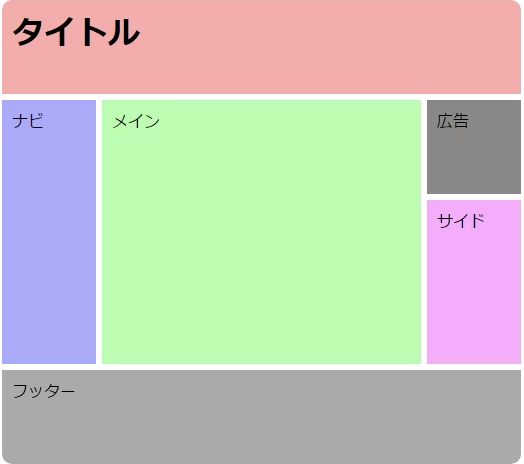
\includegraphics[width=8cm]{img/3column.png}

時間余った人は、メインの中にFlexboxを使って、記事を3つ横に並べてみよう。

参考
https://qiita.com/kura07/items/e633b35e33e43240d363











\flushright{以上}


\end{document}